\chapter{Testování: Efektivita Datastore a testování výkonu}

\section{Hlediska a způsob testování}
Pro otestování cloudu jsem vybral dvě důležitá hlediska. Prvním byla rychlost Datastore API a provádění operací: čtení, vkládání, úprava a mazání záznamů v závislosti na použitém přístupu. Testovány byly tyto možnosti: JPA, JDO a Datastore API. Druhým typem testů bylo zatížení celé aplikace a reakce cloudu. Vytvořil jsem velké množství stránek a poté jsem pomocí nástroje Apache Bench\footnote{Apache Bench je nástroj pro příkazovou řádku určený k měření výkonu serverů ---http://httpd.apache.org/docs/2.2/programs/ab.html}  posílal na App Engine požadavky. Toto testování by mělo reflektovat situaci, kdy se o dané stránce dozví v krátkém čase velký počet návštěvníků, například vyjde článek nebo reportáž, spuštění velké kampaně, anebo například použití při~propagaci jednorázové události jako jsou volby.

Všechny testy probíhaly přímo na App Engine. Sice existuje server pro lokální vývoj, ale~není zcela stejný jako cloud, jedná se jen o webový server Jetty obohacený o API služeb cloudu. Důležitým důvodem také je, že aplikace běží spolu s dalšími stránkami a navzájem se tedy ovlivňují. Cílem testu bylo simulovat co nejvíce reálné prostředí, abychom mohli odhadnout chování aplikace.  

Pokud je aplikace určitý čas neaktivní, tak se odnahraje (angl. undeploy) aby systém šetřil prostředky pro jiné aplikace. Toto nahrávání zabírá nezanedbatelný čas a mohlo by ovlivnit výsledky testů. Před každým testem byla tedy aplikace navštívena, aby bylo zajištěno, že~bude připravena a nebude potřeba ji znovu nahrávat.

\section{Testování Datastore}
Pro testování samotného uložiště jsem napsal jednoduchou aplikaci s názvem \emph{TodoList}. Tato aplikace slouží k jednoduché evidenci úkolů, ty můžeme přidávat, upravovat a mazat. Model aplikace obsahuje jednu entitu \verb|TodoEntity| a Datastore bylo naplněné několika tisíci záznamy. Pro každou z testovacích možností, tedy JPA, JDO a Datastore API, jsem vytvořil entitu s odpovídajícími anotacemi a DAO třídu \verb|TodoDAO| pro práci s Datastore. Zbytek aplikace jsem ponechal vždy stejný a při testech jsem měnil jen tuto vrstvu. Při testování byl měřen jen čistý čas operace, aby nebyly výsledky zkresleny síťovým zpožděním a dalšími faktory. Zdrojové kódy všech aplikací i s ukázkami jsou volně k dispozici\footnote{Zdrojové kódy a aplikace ke stažení  --- http://code.google.com/p/ae-cms/wiki/Aplikace}

Datastore API je optimalizováno přesně pro uložiště BigTable, používané na App Engine. Jedná se o nejpřímočařejší způsob a tak bylo očekáváno, že i tento způsob práce vyjde z testů nelépe. JPA a JDO používají anotace pro zjednodušení celé práce, ale vše je vykoupeno nutností tato data zpracovávat a převádět. To samozřejmě celou práci zpomaluje a dá se očekávat, že tyto přístupy vyjdou z testu rychlosti práce podobně, ale pomaleji než Datastore API.

První kolo testování probíhalo v odpoledních hodinách a kvůli vlivu ostatních aplikací byly některé výsledky výrazně odlišné, což celé porovnání zkreslovalo. Proto byly testy provedeny znovu kolem půlnoci našeho času, kde k takto výrazným odchylkám nedocházelo. Google má několik datacenter a vybírá, na které a na kolik z nich bude aplikace nahrána. Před dvěma lety měl App Engine datacentra dvě , jedno na východním a druhé na západním pobřeží USA, nyní je velice pravděpodobné, že má datacenter více, ale přesný počet a polohu Google nezveřenil. Vliv ostatních aplikací byl u některých testů znatelný i v noci. App Engine poskytuje statistiky využití svých služeb s grafy a dostupností přehledně zobrazené po dnech, vše je na  adrese: \verb|http://code.google.com/status/appengine/|.

\section{Test výběru}
Prvním testem bylo vybrání 1000 entit z Datastore pomocí všech způsobů. Výsledky jsou vidět v tabulce \ref{tab:select} a v grafu \ref{fig:select} Pro vybírání záznamů z uložiště je jasným favortiem Datastore API, toto rozhraní je pro výběr optimalizován, jelikož výběr bývá u většiny aplikací několikanásobně častější než ostatní operace. Na druhém místě se umístil přístup pomocí JPA a o něco pomalejší je JDO.

\begin{table}[h]
\centering
\caption{Tabulka porovnání výběru 1~000 entit (časy [ms])}\label{tab:select}
\begin{tabular}{|l|r|r|r|r|r|r|r|r|r|r|r|}
   \hline
číslo testu	& 1		& 2		& 3		& 4		& 5		& 6		& 7		& 8		& 9		& 10		& průměr \\
   \hline
Datastore API	& 1591	& 1649	& 1736	& 1708	& 2292	& 1752	& 1768	& 1645	& 1738	& 1645	& 1752 \\
JPA	& 2677	& 2438	& 2518	& 2345	& 2321	& 2337	& 2253	& 2304	& 2203	& 2346	& 2374 \\
JDO	& 2447	& 2345	& 2341	& 2619	& 2799	& 2912	& 2581	& 2632	& 2411	& 2192	& 2528 \\
   \hline
\end{tabular}
\end{table}

\begin{figure}[h]
\begin{center}
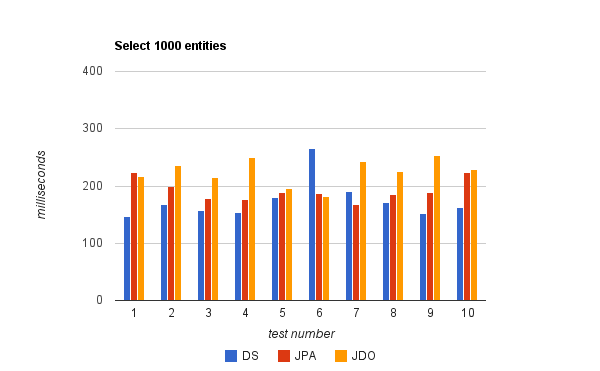
\includegraphics[width=6.5in]{figures/select.png}
\caption{Graf porovnání výběru 1~000 entit}
\label{fig:select}
\end{center}
\end{figure}

\section{Test vkládání}
Pro vkládaní záznamů již nejsou výsledky tolik rozdílné. Vítězem je znovu Datastore API, ale hned v těsném závěsu se umístil přístup pomocí JDO a hned za ním JPA (viz tabulka \ref{tab:insert} a graf \ref{fig:insert}). 

\begin{table}[h]
\centering
\caption{Tabulka porovnání vkládání 100 entit (časy [ms])}\label{tab:insert}
\begin{tabular}{|l|r|r|r|r|r|r|r|r|r|r|r|}
   \hline
číslo testu	& 1		& 2		& 3		& 4		& 5		& 6		& 7		& 8		& 9		& 10		& průměr \\
   \hline
Datastore API	& 2421	& 1931	& 1810	& 1663	& 1637	& 1445	& 1543	& 1488	& 1585	& 1578	& 1710 \\
JPA	& 2429	& 2178	& 2120	& 2044	& 2255	& 2023	& 1961	& 2698	& 1973	& 1878	& 2156 \\
JDO	& 1891	& 1881	& 1851	& 1696	& 1764	& 2012	& 1781	& 1834	& 1765	& 1826	& 1830 \\
   \hline
\end{tabular}
\end{table}

\begin{figure}[h]
\begin{center}
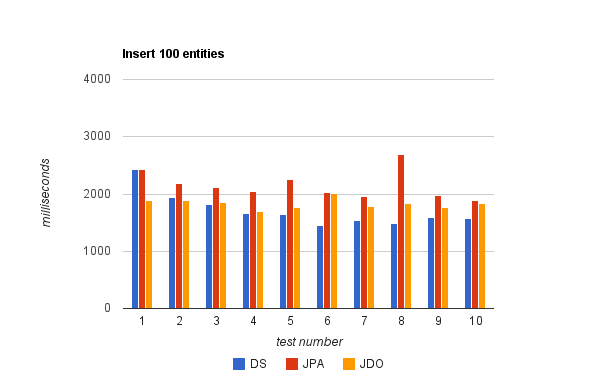
\includegraphics[width=6.5in]{figures/insert.png}
\caption{Graf porovnání vkládání 100 entit}
\label{fig:insert}
\end{center}
\end{figure}

\section{Test úprava}

Při úpravě entity překvapivě JPA i JDO pracovaly rychleji než Datastore API. Nejrychlejší byl nyní JDO přístup. Pomalost Datastore API byla pravděpodobně způsobena implementací DAO vrstvy. Nejdříve byla entita vybrána z databáze, poté byly změněny hodnoty a následně celá entita znovu uložena. Výsledky jsou v tabulce \ref{tab:update} a grafu \ref{fig:update}.

\begin{table}[h]
\centering
\caption{Tabulka porovnání úpravy 100 entit  (časy [ms])}\label{tab:update}
\begin{tabular}{|l|r|r|r|r|r|r|r|r|r|r|r|}
   \hline
číslo testu	& 1		& 2		& 3		& 4		& 5		& 6		& 7		& 8		& 9		& 10		& průměr \\
   \hline
Datastore API	& 2309	& 5809	& 2442	& 2245	& 2283	& 2199	& 3407	& 2908	& 2085	& 2217	& 2501 \\
JPA	& 2139	& 2171	& 2219	& 2135	& 2026	& 2234	& 1997	& 6232	& 2191	& 2181	& 2162 \\
JDO	& 1704	& 1775	& 1950	& 1703	& 1735	& 1870	& 1752	& 1711	& 1889	& 1719	& 1769 \\
   \hline
\end{tabular}
\end{table}

\begin{figure}[h]
\begin{center}
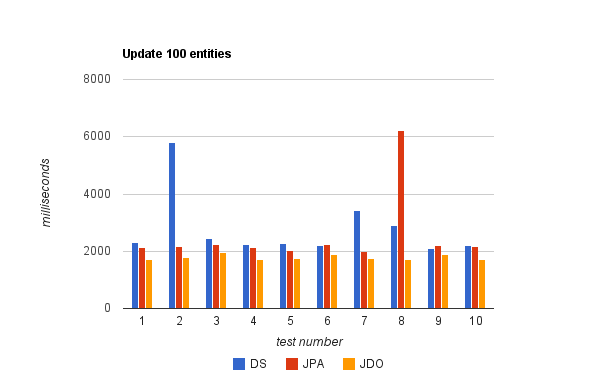
\includegraphics[width=6.5in]{figures/update.png}
\caption{Graf porovnání úpravy 100 entit}
\label{fig:update}
\end{center}
\end{figure}


\section{Test mazání}

Pro mazání bylo Datastore API výrazně rychlejší. JPA a JDO na tom byly s rychlostí podobně, ale JPA vyšlo o něco lépe. Výsledky viz tabulka \ref{tab:delete} a graf \ref{fig:delete}.

\begin{table}[h]
\centering
\caption{Tabulka porovnání mazání 100 entit (časy [ms])}\label{tab:delete}
\begin{tabular}{|l|r|r|r|r|r|r|r|r|r|r|r|}
   \hline
číslo testu	& 1		& 2		& 3		& 4		& 5		& 6		& 7		& 8		& 9		& 10		& průměr \\
   \hline
Datastore API	& 1591	& 1649	& 1736	& 1708	& 2292	& 1752	& 1768	& 1645	& 1738	& 1645	& 1752 \\
JPA	& 2677	& 2438	& 2518	& 2345	& 2321	& 2337	& 2253	& 2304	& 2203	& 2346	& 2374 \\
JDO	& 2447	& 2345	& 2341	& 2619	& 2799	& 2912	& 2581	& 2632	& 2411	& 2192	& 2528 \\
   \hline
\end{tabular}
\end{table}

\begin{figure}[h]
\begin{center}
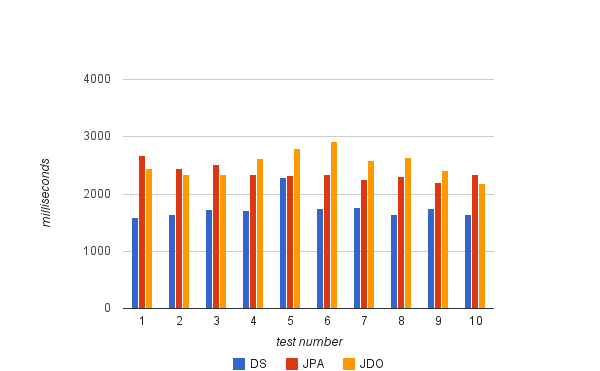
\includegraphics[width=6.5in]{figures/delete.png}
\caption{Graf porovnání mazání 100 entit}
\label{fig:delete}
\end{center}
\end{figure}

\section{Porovnání výsledků testů práce s Datastore}
Celkově tedy v testech dopadlo dle očekávání nejrychleji Datastore API. Jedná se o přímočarý přístup k uložišti a nestará se o další transformace. Bohužel tato rychlost je vykoupena složitější implementací a odlišným způsobem práce. Při úpravě dat bylo podle výsledků testů Datastore API nejpomalejší, to bylo způsobeno odlišným způsobem práce, kdy jsme objekt vybírali z databáze a poté upravovali. Je to dáno rozdílností práce s Datastore API oproti JPA a JDO, pravděpodobně by se nám pomocí optimalizací podařilo dostat výsledky na stejnou úroveň jako ostatní dvě řešení. Každopádně i přesto je Datastore API jasným vítězem. JPA a JDO jsou na tom podle provedených testů výkonnostně podobně. JPA vyniká v rychlosti při čtení a mazání, kdežto JDO je rychlejší při vkládání a úpravě. Práce s těmito dvěma přístupy je podobná a záleží tedy hlavně na zvyku a zkušenosti programátora, kterou si vybere. Při velkém počtu čtení z Datastore oproti ostatním operacím je z těchto dvou přístupů z hlediska rychlosti vhodnější využít právě JPA.


\section{Testování výkonu}
Pro testování výkonu bylo na stránku posláno velké množství požadavků a cílem bylo zjistit, jak bude celá aplikace na takovýto nápor reagovat. Aby nešlo jen o jednoduché vybírání jedné stránky, tak bylo do aplikace vloženo celkem 10~000 stránek. Každá ze stránek má nastavenou svoji šablonu, takže ta se při sestavování odpovědi musela z Datastore získat také. Celá tato aplikace je veřejně přístupná na webu na adrese: \verb|http://slim3cms.appspot.com|.


Samotné testování probíhalo pomocí programu Apache Bench (ab). Jedná se o jednoduchý program pro příkazovou řádku, kde specifikujeme adresu serveru, počet požadavků a počet souběžných požadavků, které se mají na server odeslat. Program poté vypíše výsledky testů. Vždy před testem byla aplikace navštívena, aby byla alespoň jedna instance aktivní.

\lstset{language=bash}
\lstset{numbers=none}
\lstset{frame=none}
\begin{lstlisting}[caption={Testování 1000 požadavků se 100 souběžnými spojeními},label=lst:testOne,belowcaptionskip=0.4cm]
ab -n 1000 -c 100 http://slim3cms.appspot.com
\end{lstlisting}

Při prvním testu bylo posláno dohromady 1~000 požadavků se 100 současnými připojeními (viz~zdrojový kód \ref{lst:testOne}). Celý test trval 16,656 sekund a po skončení testu bylo na App Engine nahráno 13 aktivních instancí.

Při druhém testu byly parametry stejné. Tento test následoval hned po prvním, kdy byla většina instancí stále aktivních a trval test pouhých 8,619 sekund Což je skoro polovina původního času, to díky již připraveným instancím, které stihly rychle zareagovat na vzniklý nápor. Na konci testu bylo aktivních 20 instancí.

\begin{lstlisting}[caption={Testování 4000 požadavků s 1000 souběžnými spojeními},label=lst:testThree,belowcaptionskip=0.4cm]
ab -n 4000 -c 1000 http://slim3cms.appspot.com
\end{lstlisting}

Při posledním testu bylo posláno 4~000 požadavků s 1~000 současnými připojeními (viz~zdrojový kód \ref{lst:testThree}) a byl spuštěn krátký čas po druhém testování. Celý test trval 15,748 sekund a~po~skončení bylo aktivních celkem 30 instancí aplikace.

\begin{table}[h]
\centering
\caption{Tabulka porovnání zátěže}\label{tab:requestTest}
\begin{tabular}{|r|r|r|r|}
   \hline
požadavků	& spojení	& instancí	& doba testu [s]	\\
   \hline
1000			& 100	& 13		& 16,656	\\
1000			& 100	& 20		& 8,619 	\\
4000			& 1000	& 30		& 15,748	 \\
   \hline
\end{tabular}
\end{table}

Výlsedky testů jsou zobrazeny v tabulce \ref{tab:requestTest}. Více požadavků se mi bohužel odeslat nepodařilo, jelikož při překročení 4~000 požadavků program Apache Bench nechtěl test dokončit. Problém nebude u App Engine, protože se stejný problém projevoval i u jiných serverů. Testování jsem prováděl na 10~Mb domácí lince. Kvóty byly tímto testem poznamenány minimálně až na procesorový čas. Toho bylo spotřebováno 1,24~hodiny, tedy 19\% z celkových 6,5~hodiny za~den. Jednalo se ale i o zdroje spotřebované při vkládání 10.000 entit do aplikace, takže na samotný test připadá zhruba 1 hodina procesorového času.

Test by mohl být zajímavější, pokud by App Engine dostával požadavky z více současně spuštěných programu Apache Bench z rozdílných sítí. Dalo by se předpokládat, že by byly nahrány další instance podle potřeby a požadavky by byly rovnoměrně rozdistribuovány. Ke znatelnému zatížení App Engine by byla potřeba mnohem větší infrastruktura a zdroje, příkladem může být právě aplikace www.officialroyalwedding2011.org (viz kapitola 2.9), kde~bylo požadavků mnohonásobně více a cloud si s nimi dokázal bez problému poradit.

Velkého zatížení naší aplikace se tedy na App Engine nemusíme bát, cloud se s nimi dokáže správně vypořádat a rozdělit zátěž. Jediné co se může stát je, že přesáhneme některou z kvót, ale ty lze jednoduše dokoupit. Velkou výhodou je samostatná správa počtu instancí podle potřeby, App Engine takto dokáže efektivně využít hardwarové zdroje.
